\documentclass[11pt,a4paper]{article}

\usepackage{amsmath,amssymb,amsthm}
\usepackage{bm}
\usepackage{booktabs}
\usepackage{array}
\usepackage{geometry}
\usepackage{hyperref}
\usepackage{microtype}
\usepackage{parskip}
\usepackage{tikz}
\usetikzlibrary{arrows.meta}

\geometry{margin=2.5cm}

\hypersetup{
    colorlinks=true,
    linkcolor=blue,
    citecolor=blue,
    urlcolor=blue,
}

\newcommand{\vx}{\mathbf{x}}
\newcommand{\vg}{\mathbf{g}}
\newcommand{\vv}{\mathbf{v}}
\newcommand{\vJ}{\mathbf{J}}
\newcommand{\vV}{\mathbf{V}}
\newcommand{\mLambda}{\boldsymbol{\Lambda}}
% \Omega is already defined by LaTeX
\newcommand{\norm}[1]{\left\|#1\right\|}

\title{Dose-Weighted Sobel Metrics and Structure-Tensor-Based\\
       Edge Orientation for Proton Therapy Complexity Analysis}
\author{ADoTA Project}
\date{\today}

\begin{document}
\maketitle

\begin{abstract}
We define a set of heterogeneity metrics based on the 3-D Sobel edge filter
applied to CT Hounsfield-unit volumes in the neighbourhood of the Bragg peak.
Two extensions over a plain gradient-magnitude summary are introduced.
First, every voxel's contribution is weighted by the local dose, so that tissue
interfaces outside the irradiated region are discounted.
Second, rather than discarding the directional information carried by the
gradient vector, we aggregate gradient directions via the \emph{dose-weighted
structure tensor}, whose eigendecomposition yields the dominant edge normal and
a set of interpretable scalar shape descriptors.
These descriptors are intended as predictors of model error in
machine-learning-based proton dose prediction.
In this document they are positioned as candidate difficulty estimators inside
an \emph{active beamlet mining} pipeline that selects beamlet-induced CT
patches for expensive Monte Carlo dose calculation
(Section~\ref{sec:framework}).
\end{abstract}

\tableofcontents
\newpage

% ---------------------------------------------------------------------------
\section{Research Framework: Active Beamlet Mining}
\label{sec:framework}
% ---------------------------------------------------------------------------

The Sobel and structure-tensor metrics developed in the remainder of this
document are intended as a building block of a larger active-learning
pipeline for proton dose calculation.
Before introducing the technical material we state the broader research
formulation in which these metrics will be embedded; the dose-weighted
Sobel descriptors defined in
Section~\ref{sec:dw_metrics} onward instantiate the abstract
\emph{difficulty estimator} that appears in the formulation below.

\subsection{Clean Research Formulation: Active Beamlet Mining}

Let \(I \in \mathbb{R}^{D \times H \times W}\) denote a 3D CT image (depth-first
axis ordering, consistent with Section~\ref{sec:notation}) and let
\(M_{\theta}\) denote a trained, but imperfect, deep-learning-based dose
calculation model. The objective is to improve \(M_{\theta}\) by actively
selecting beamlet-induced CT patches for which expensive Monte Carlo dose
calculation is expected to provide the highest training value.

A proton beamlet is parameterized as
\[
b = (\mathbf{d}, u, v),
\]
where \(\mathbf{d} \in S^2\) is the beam direction and \((u,v)\) defines the
lateral beamlet position in the plane orthogonal to \(\mathbf{d}\). The space of
feasible beamlets for a given CT image is denoted by
\[
\mathcal{B}(I).
\]

\begin{figure}[h!]
\centering
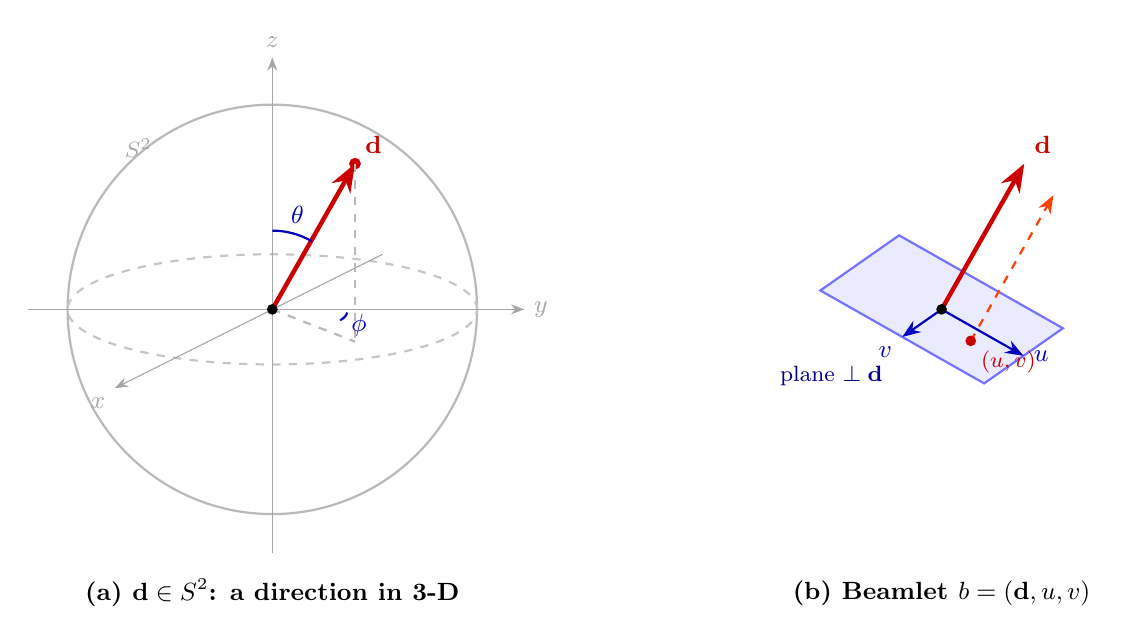
\begin{tikzpicture}[>=Stealth, font=\small, thick]

%% =============== Panel (a): the unit 2-sphere S^2 ===============
\begin{scope}[xshift=0cm]

  % --- Sphere silhouette and equator ---
  \draw[gray!55] (0,0) circle (2.6cm);
  \draw[gray!45, dashed] (0,0) ellipse (2.6cm and 0.7cm);

  % --- Axes ---
  \draw[->, gray!70, thin] (-3.1, 0) -- (3.2, 0)   node[right] {$y$};
  \draw[->, gray!70, thin] (0, -3.1) -- (0, 3.2)   node[above] {$z$};
  \draw[->, gray!70, thin] (1.4, 0.7) -- (-2.0, -1.0) node[below left] {$x$};

  % --- Direction vector d ---
  \coordinate (Oa) at (0, 0);
  \coordinate (Da) at (1.05, 1.85);
  \coordinate (Pa) at (1.05, -0.41);

  \draw[->, ultra thick, red!80!black] (Oa) -- (Da);
  \node[red!80!black, above right] at (Da) {$\mathbf{d}$};
  \filldraw[red!80!black] (Da) circle (1.7pt);

  % --- Projection helpers ---
  \draw[gray!55, dashed] (Da) -- (Pa);
  \draw[gray!55, dashed] (Oa) -- (Pa);

  % --- Polar angle theta ---
  \draw[blue!75!black, thick] (0, 1.0) arc (90:60:1.0);
  \node[blue!75!black] at (0.32, 1.20) {$\theta$};

  % --- Azimuthal angle phi (in xy-plane) ---
  \draw[blue!75!black, thick]
        (0.95, -0.04) arc (-2:-25:0.95cm and 0.255cm);
  \node[blue!75!black] at (1.10, -0.20) {$\phi$};

  % --- Origin and S^2 label ---
  \filldraw (Oa) circle (1.5pt);
  \node[gray!70, font=\footnotesize] at (-1.7, 2.05) {$S^2$};

  % --- Panel title ---
  \node[align=center, font=\small\bfseries] at (0, -3.6)
    {(a) $\mathbf{d} \in S^2$: a direction in 3-D};

\end{scope}

%% =============== Panel (b): full beamlet b = (d, u, v) ===============
\begin{scope}[xshift=8.5cm]

  \coordinate (Ob) at (0, 0);
  \coordinate (Db) at (1.05, 1.85);

  % --- Lateral plane perpendicular to d ---
  \filldraw[blue!8, draw=blue!55, thick]
    (-0.54, 0.94) -- (-1.54, 0.24) -- (0.54, -0.94) -- (1.54, -0.24) -- cycle;

  % --- d arrow (central beam direction) ---
  \draw[->, ultra thick, red!80!black] (Ob) -- (Db);
  \node[red!80!black, above right] at (Db) {$\mathbf{d}$};

  % --- u, v axes within the plane ---
  \draw[->, blue!75!black, thick] (Ob) -- (1.04, -0.59);
  \node[blue!75!black, right] at (1.04, -0.59) {$u$};

  \draw[->, blue!75!black, thick] (Ob) -- (-0.5, -0.35);
  \node[blue!75!black, below left] at (-0.5, -0.35) {$v$};

  % --- Offset point in plane and pencil beam through it ---
  \coordinate (Pb) at (0.37, -0.40);
  \draw[->, thick, red!50!orange, dashed] (Pb) -- (1.42, 1.45);
  \filldraw[red!80!black] (Pb) circle (1.5pt);
  \node[red!80!black, font=\footnotesize, below right] at (Pb) {$(u, v)$};

  % --- Origin marker ---
  \filldraw (Ob) circle (1.5pt);

  % --- Plane label ---
  \node[blue!55!black, font=\footnotesize] at (-1.4, -0.85)
    {plane $\perp \mathbf{d}$};

  % --- Panel title ---
  \node[align=center, font=\small\bfseries] at (0, -3.6)
    {(b) Beamlet $b = (\mathbf{d}, u, v)$};

\end{scope}

\end{tikzpicture}
\caption{Two views of the proton-beamlet parametrisation.
\textbf{(a)}~The unit 2-sphere $S^2 = \{\mathbf{d} \in \mathbb{R}^3 :
\|\mathbf{d}\|_2 = 1\}$ is the space of beam directions: every point on its
surface is one unit vector $\mathbf{d}$ from the origin, and conversely every
direction in 3-D space is one such point.  Two angles parametrise
$\mathbf{d}$ — the polar angle $\theta \in [0,\pi]$ from the $z$-axis and
the azimuthal angle $\phi \in [0,2\pi)$ in the $xy$-plane — confirming that
$\mathbf{d}$ has two degrees of freedom.
\textbf{(b)}~Once $\mathbf{d}$ is chosen, the lateral position $(u, v)$ fixes
the pencil beam within the plane orthogonal to $\mathbf{d}$ (blue
parallelogram).  The dashed orange ray is the actual pencil beam: a line
parallel to $\mathbf{d}$ passing through the offset point $(u, v)$.  Total
degrees of freedom: $2 + 2 = 4$ per beamlet.}
\label{fig:S2_beamlet}
\end{figure}

Given a beamlet \(b \in \mathcal{B}(I)\), a raytracing operator extracts a
beam-aligned CT patch
\[
x_b = R(I,b),
\]
where \(R\) denotes the patch extraction operator. The patch \(x_b\) represents
the local anatomical region through which the proton beamlet travels and is
expressed in \emph{beamlet coordinates}: axis~$0$ is the depth direction along
\(\mathbf{d}\), and axes~$1,2$ lie in the lateral plane orthogonal to
\(\mathbf{d}\).  All Sobel and structure-tensor metrics introduced in
Sections~\ref{sec:notation}--\ref{sec:scalar} operate on \(x_b\) in this
beamlet-aligned frame.

Assume that a difficulty estimator
\[
\Delta(x_b)
\]
is available. This estimator assigns a scalar score to each extracted patch,
reflecting the expected difficulty of the patch for the current dose calculation
model \(M_{\theta}\).

The active learning problem is then formulated as the selection of a subset of
beamlets
\[
S^\star = \{b_1,\ldots,b_K\} \subset \mathcal{B}(I)
\]
whose corresponding patches should be evaluated with Monte Carlo simulation and
added to the training database.

A naive strategy would select the beamlets with the largest difficulty scores:
\[
S^\star
=
\arg\max_{S \subset \mathcal{B}(I), \ |S|=K}
\sum_{b \in S} \Delta(x_b).
\]
However, this may result in selecting many redundant beamlets that traverse
similar anatomical regions.

To control redundancy and promote variability, we introduce a patch embedding
function
\[
E : \mathcal{X} \rightarrow \mathbb{R}^m,
\]
which maps each beamlet-induced patch \(x_b\) to a low-dimensional latent
representation
\[
z_b = E(x_b).
\]

The set
\[
\mathcal{M}_I
=
\left\{
E(R(I,b)) : b \in \mathcal{B}(I)
\right\}
\]
defines a CT-specific beamlet-patch manifold. This manifold represents the
geometry of all candidate beamlet-induced patches for the given CT image.

Let \(\mathcal{D}_{\mathrm{train}}\) denote the current training database,
containing previously sampled beamlet patches. The novelty of a candidate
beamlet \(b\) with respect to the existing training data is defined as
\[
N(b)
=
\min_{q \in \mathcal{D}_{\mathrm{train}}}
\left\|
E(x_b) - E(x_q)
\right\|_2.
\]

For a partially selected set \(S\) we additionally need a measure of how
similar a candidate beamlet \(b\) is to those already chosen.  Let
\(z_b = E(x_b) = E(R(I,b))\) denote the latent code of patch \(x_b\).  We
use the Gaussian (RBF) similarity \emph{kernel} between latent codes,
\[
   k(z, z') = \exp\!\left(-\frac{\|z - z'\|_2^2}{\sigma^2}\right) \in [0, 1],
\]
where \(\sigma > 0\) is the kernel \emph{bandwidth}.  This is the same RBF
kernel used in support-vector machines and Gaussian-process regression;
\(\sigma\) is \emph{not} the standard deviation of a probability
distribution but a length-scale parameter in the embedding space,
controlling how rapidly the similarity score decays with distance:
\(k = 1\) at zero distance, \(k \approx 0.37\) at distance \(\sigma\), and
\(k \to 0\) as the distance grows large.

\paragraph{Why a bounded kernel for redundancy but a raw distance for novelty?}
The novelty term \(N(b)\) only has to be \emph{monotone} in distance —
greater distance from the training database is always better — so the raw
\(L_2\) distance suffices.  The redundancy term, by contrast, enters the
acquisition function with a fixed weight \(\lambda\) alongside
\(\Delta(x_b)\) and \(N(b)\), each of which has its own intrinsic scale.
If redundancy were the raw squared distance to the nearest already-selected
beamlet its magnitude would depend on the (arbitrary) scale of the embedding
\(E\), and \(\lambda\) would have to be re-tuned every time \(E\) changes.
Mapping distance through \(k\) bounds the redundancy contribution to
\([0, 1]\) and makes \(\lambda\) directly interpretable as the weight
assigned to a perfect duplicate.

\paragraph{Set-level objective.}
The principled active beamlet mining objective is to maximise total
per-beamlet utility while penalising pairwise similarity within the
selected set:
\[
   S^\star
   = \arg\max_{S\, \subset\, \mathcal{B}(I),\ |S|=K}
     \;\sum_{b \in S}\bigl[\Delta(x_b) + \gamma\, N(b)\bigr]
     \;-\; \lambda\!\!\!\!\sum_{\{b_i, b_j\}\, \subset\, S}\!\!\!\!
              k(z_{b_i}, z_{b_j}),
\]
where \(\sum_{\{b_i,b_j\} \subset S}\) denotes a sum over \emph{unordered
pairs} of distinct beamlets in \(S\), and \(\gamma \geq 0\),
\(\lambda \geq 0\) trade off novelty and diversity against difficulty.
This set-level form is the defining objective: it is the standard
Gaussian-kernel diversification criterion and, with appropriate
normalisation, connects to determinantal-point-process active learning.

\paragraph{Greedy approximation.}
Solving the set-level problem exactly is combinatorial.  We use a greedy
approximation: starting from \(S_0 = \emptyset\), at step \(t\) we add the
candidate that maximises a per-element acquisition function,
\[
   A(b;\, S_{t-1})
   = \Delta(x_b) + \gamma\, N(b) - \lambda\, R_{\mathrm{red}}(b,\, S_{t-1}),
\]
where the redundancy contribution is taken to be the kernel similarity of
\(b\) to its closest already-selected neighbour,
\[
   R_{\mathrm{red}}(b,\, S)
   = \max_{b_j \in S}\, k(z_b, z_{b_j}).
\]
The greedy step is then
\[
   b_t^\star
   = \arg\max_{b\, \in\, \mathcal{B}(I)\, \setminus\, S_{t-1}}
     A(b;\, S_{t-1}),
   \qquad
   S_t = S_{t-1} \cup \{b_t^\star\},
\]
iterated until \(|S_t| = K\).

\paragraph{Relation between the set-level objective and the greedy surrogate.}
The exact marginal contribution of adding \(b\) to \(S_{t-1}\) under the
set-level pairwise penalty is the \emph{sum}
\(\sum_{b_j \in S_{t-1}} k(z_b, z_{b_j})\).  The max-version used in
\(R_{\mathrm{red}}\) replaces this sum with its single largest summand and
is therefore a stricter, more conservative diversity heuristic: a candidate
is penalised by its closest neighbour in \(S\) alone, so a near-duplicate
of any one already-selected beamlet is rejected even when far from all the
others.  The max form is the default because it is cheaper to evaluate
(\(O(|S_{t-1}|)\) per candidate) and produces well-spread selections in
practice; the corresponding sum-version surrogate
\(R_{\mathrm{red}}^{\Sigma}(b, S) = \sum_{b_j \in S} k(z_b, z_{b_j})\),
which is the exact greedy marginal of the set-level objective, will be
evaluated as an alternative.

The selected beamlets define the set of patches
\[
\mathcal{X}_{\mathrm{MC}}
=
\left\{
x_b = R(I,b) : b \in S^\star
\right\},
\]
for which Monte Carlo dose calculations are performed. The resulting labeled
samples are added to the training database:
\[
\mathcal{D}_{\mathrm{train}}^{\mathrm{new}}
=
\mathcal{D}_{\mathrm{train}}
\cup
\left\{
(x_b, D_b^{\mathrm{MC}}) : b \in S^\star
\right\}.
\]

The dose calculation model is then updated by minimizing the supervised training
objective
\[
\theta^\star
=
\arg\min_{\theta}
\sum_{(x,D^{\mathrm{MC}}) \in \mathcal{D}_{\mathrm{train}}^{\mathrm{new}}}
\mathcal{L}
\left(
M_{\theta}(x),
D^{\mathrm{MC}}
\right).
\]

This formulation defines active beamlet mining as a geometry-aware acquisition
problem over the space of feasible proton beamlets. The manifold representation
is not constructed over the CT image itself, but over the set of beamlet-induced
patches generated from the CT image:
\[
\mathcal{M}_I
=
\left\{
E(R(I,b)) : b \in \mathcal{B}(I)
\right\}.
\]
The acquisition process therefore prioritizes beamlets that are simultaneously
difficult for the current model, novel with respect to the existing training
database, and non-redundant with respect to already selected beamlets.

\subsection{Connection to the Remainder of This Document}
\label{sec:framework_to_sobel}

The remainder of this document develops one concrete realisation of the
difficulty estimator $\Delta(x_b)$ defined above.
For each beamlet-induced patch $x_b = R(I,b)$ a vector of dose-weighted
Sobel and structure-tensor descriptors,
\[
    \boldsymbol{\phi}(x_b)
    = \bigl(\bar{S}_{dw}(x_b),\;
            A(x_b),\;
            \theta(x_b),\;
            E_{\text{total}}(x_b)\bigr) \in \mathbb{R}^4,
\]
is computed (Sections~\ref{sec:dw_metrics}--\ref{sec:scalar}), each component
isolating a distinct, physically interpretable aspect of the local tissue
geometry traversed by the beamlet.
The difficulty estimator is then any scalar function of these descriptors,
\[
    \Delta(x_b) = h\bigl(\boldsymbol{\phi}(x_b)\bigr).
\]
Three reasonable forms of $h$ will be considered:
\begin{enumerate}
    \item a \emph{single descriptor}, e.g.\ $\theta(x_b)$ alone, motivated
          by its direct link to range uncertainty
          (Section~\ref{sec:angle});
    \item a \emph{hand-tuned weighted sum} of components of
          $\boldsymbol{\phi}$ chosen on physical grounds; or
    \item a \emph{regression model} (e.g.\ a small MLP, random forest, or
          regularised linear model) fitted to predict the observed gamma
          pass rate from $\boldsymbol{\phi}$ across the existing training
          set.
\end{enumerate}
The empirical comparison of Method DW and Method TH
(Section~\ref{sec:comparison}) supplies the evidence required to choose
between weighted and threshold-masked variants of each descriptor before
the form of $h$ is finalised.

The patch embedding $E(x_b)$ used for novelty $N(b)$ and redundancy
$R_{\mathrm{red}}(b,S)$ is logically distinct from $\Delta(x_b)$ and may use a
different representation: a learned encoder (for example the bottleneck of
$M_\theta$ itself), a pre-trained 3-D CNN, or the descriptor vector
$\boldsymbol{\phi}(x_b)$ itself.
This document does not commit to a specific embedding; that choice is
deferred to a separate methodological note.

% ---------------------------------------------------------------------------
\section{Notation and Setup}
\label{sec:notation}
% ---------------------------------------------------------------------------

Let $I(\vx)$ denote the CT intensity (Hounsfield units) at voxel
$\vx = (z,y,x) \in \mathbb{Z}^3$, and let $d(\vx) \geq 0$ denote the
ground-truth absorbed dose at the same voxel.
\textbf{Notational convention.}  In Section~\ref{sec:framework} the symbol
$I$ denotes the full patient CT image; here and in subsequent sections we
re-use $I$ for the \emph{beam-aligned patch} $x_b = R(\,\cdot\,,b)$ produced
by the raytracing operator, with the beamlet index $b$ suppressed for
notational economy.  With this convention axis~$0$ ($z$) is the depth
direction along the beam, and axes~$1,2$ ($y,x$) span the lateral plane
orthogonal to it.
Physical coordinates are obtained by multiplying voxel indices by the
isotropic voxel spacing $(\delta_z, \delta_y, \delta_x)$ in mm.

The \emph{Bragg-peak location} $\vx_{BP}$ is the voxel that maximises the
depth-integrated dose in the axial direction:
\begin{equation}
    \vx_{BP} = \arg\max_{\vx}\; d(\vx).
\end{equation}

The \emph{analysis sphere} of radius $R$ (mm) centred on $\vx_{BP}$ is
\begin{equation}
    \Omega_R
    = \Bigl\{\vx \in \mathbb{Z}^3 :
        (z - z_{BP})^2\delta_z^2
      + (y - y_{BP})^2\delta_y^2
      + (x - x_{BP})^2\delta_x^2
      \leq R^2 \Bigr\}.
\end{equation}

% ---------------------------------------------------------------------------
\section{Three-Dimensional Sobel Gradient}
% ---------------------------------------------------------------------------

The 3-D Sobel operator approximates the partial derivative of $I$ along each
axis by convolving with axis-specific kernels.
The resulting gradient vector at voxel $\vx$ is
\begin{equation}
    \vg(\vx)
    = \begin{pmatrix} G_z(\vx) \\ G_y(\vx) \\ G_x(\vx) \end{pmatrix},
    \qquad
    \norm{\vg(\vx)} = \sqrt{G_z^2 + G_y^2 + G_x^2}.
\end{equation}

The unit-norm gradient, wherever $\norm{\vg} > 0$, is the
\emph{edge normal}:
\begin{equation}
    \hat{n}(\vx) = \frac{\vg(\vx)}{\norm{\vg(\vx)}}.
\end{equation}

\subsection*{Why gradient direction matters}

The Sobel gradient magnitude $\norm{\vg}$ captures only \emph{how strong} a
tissue interface is, not \emph{how it is oriented}.
In proton therapy, the range of a pencil beam is sensitive to the material it
traverses along the beam axis (here $\hat{z}$).
An interface whose normal is parallel to $\hat{z}$ (i.e.\ the interface is
perpendicular to the beam) perturbs the water-equivalent path length and
therefore the Bragg-peak depth.
An interface whose normal is orthogonal to $\hat{z}$ (i.e.\ the interface
runs along the beam) causes lateral heterogeneity but less range shift.
Capturing the dominant edge orientation is therefore physically motivated.

% ---------------------------------------------------------------------------
\section{Dose-Weighted Sobel Metrics}
\label{sec:dw_metrics}
% ---------------------------------------------------------------------------

\subsection{Motivation}

The existing implementation aggregates $\norm{\vg}$ uniformly over
$\Omega_R$, treating every voxel equally regardless of whether it receives
dose.
A tissue interface far from any isodose surface does not affect dose
complexity, so its gradient should not inflate the heterogeneity score.
We replace uniform aggregation with dose weighting.

\subsection{Dose-Weighted Mean Gradient Magnitude}

\begin{equation}
    \boxed{
    \bar{S}_{dw}
    = \frac{\displaystyle\sum_{\vx \in \Omega_R} d(\vx)\,\norm{\vg(\vx)}}
           {\displaystyle\sum_{\vx \in \Omega_R} d(\vx)}
    }
    \label{eq:dw_mean}
\end{equation}

This is a proper weighted average of edge strength, where the weights are the
local dose values.
Voxels with $d(\vx) = 0$ contribute nothing; voxels near the dose maximum
contribute most.

The metric is defined for $\sum_{\vx \in \Omega_R} d(\vx) > 0$; if the
sphere contains no dose it defaults to zero.

\subsection{Relationship to the Existing Metric}

The current unweighted mean corresponds to setting $d(\vx) = 1$ for all
$\vx \in \Omega_R$:
\begin{equation}
    \bar{S}_{unweighted}
    = \frac{1}{|\Omega_R|}\sum_{\vx \in \Omega_R} \norm{\vg(\vx)}.
\end{equation}
Equation~\eqref{eq:dw_mean} is a strict generalisation.

\subsection{Method TH: Threshold-Masked Mean}
\label{sec:method_th}

The second approach replaces continuous dose weighting with a binary
mask defined by a global dose threshold.
Let $d_{\mathrm{grid}} = \max_{\vx \in \mathcal{V}} d(\vx)$ be the maximum
dose over the \emph{entire CT grid} $\mathcal{V}$ (not just inside the
sphere).
The active set at threshold $\varepsilon = 0.05$ is:
\begin{equation}
    \Omega_R^{TH}
    = \bigl\{\vx \in \Omega_R : d(\vx) \geq \varepsilon\,d_{\mathrm{grid}}\bigr\}.
    \label{eq:active_set}
\end{equation}
The threshold metric is the unweighted mean of gradient magnitudes over this
active set:
\begin{equation}
    \boxed{
    \bar{S}_{TH}
    = \frac{1}{\lvert\Omega_R^{TH}\rvert}
      \sum_{\vx \in \Omega_R^{TH}} \norm{\vg(\vx)}.
    }
    \label{eq:th_mean}
\end{equation}

All voxels inside $\Omega_R^{TH}$ contribute equally; those outside (below
5\,\% of the global dose peak) contribute nothing.
The same binary mask is applied to the structure tensor:
\begin{equation}
    \vJ_{TH}
    = \sum_{\vx \in \Omega_R^{TH}} \vg(\vx)\otimes\vg(\vx),
    \label{eq:th_tensor}
\end{equation}
from which anisotropy $A_{TH}$, beam-edge angle $\theta_{TH}$, and total
edge energy $E_{TH}$ are derived analogously to
Sections~\ref{sec:angle}--\ref{eq:total_energy}.

\paragraph{Why use the global grid maximum?}
Normalising the threshold to the whole-grid dose peak (rather than the
in-sphere peak) makes the threshold consistent across samples and physically
grounded: $0.05\,d_{\mathrm{grid}}$ corresponds to the clinical 5\,\%
isodose surface of the plan, a standard boundary used in radiotherapy
dosimetry to separate irradiated from unirradiated tissue.

\paragraph{Key difference from Method DW.}
Method DW~\eqref{eq:dw_mean} assigns each voxel a weight proportional to
its dose — a soft, continuous transition.
Method TH~\eqref{eq:th_mean} makes a hard binary decision: a voxel is either
``in'' or ``out''.
Within the active set, every voxel contributes equally regardless of whether
it sits at the dose peak or just above the threshold.

% ---------------------------------------------------------------------------
\section{Dose-Weighted Structure Tensor}
% ---------------------------------------------------------------------------

\subsection{The Cancellation Problem: Why We Cannot Average Gradient Vectors}

The Sobel operator gives us, at every voxel, an arrow whose direction is
perpendicular to the nearest tissue boundary.
A first idea would be to simply average all these arrows over the sphere to
find the ``dominant'' interface direction.
Unfortunately, this approach fails by construction.

Consider a thin bone slab passing through the centre of the sphere
(Figure~\ref{fig:cancellation}).
The slab creates two parallel interfaces: a left face (soft tissue on the
left, bone on the right) and a right face (bone on the left, soft tissue
on the right).
The Sobel gradient points from lower to higher CT intensity, i.e.\ from
soft tissue toward bone:
\begin{itemize}
    \item At the \emph{left face}, the adjacent soft tissue is to the left of
          the bone, so the gradient in that tissue region points
          \textbf{rightward} (toward the denser bone).
    \item At the \emph{right face}, the adjacent soft tissue is to the right,
          so the gradient in that tissue region points \textbf{leftward}
          (again toward the bone, but now from the opposite side).
\end{itemize}
Both gradient sets are equally strong and point in exactly opposite
directions; their sum over the sphere is zero (Figure~\ref{fig:cancellation}a).
Yet the interface is as real and as sharp as possible.
In clinical practice this scenario — a bone plate (e.g.\ a rib or the iliac
crest) running across the beam path — is one of the most relevant sources of
range uncertainty in proton therapy.

This is not a numerical quirk; it is an unavoidable consequence of the fact
that a gradient vector is a \emph{signed} quantity.
Any method that sums signed vectors will exhibit this cancellation whenever
the sphere contains an interface that is symmetric about its centre, which is
precisely the situation we care about most.

\begin{figure}[h!]
\centering
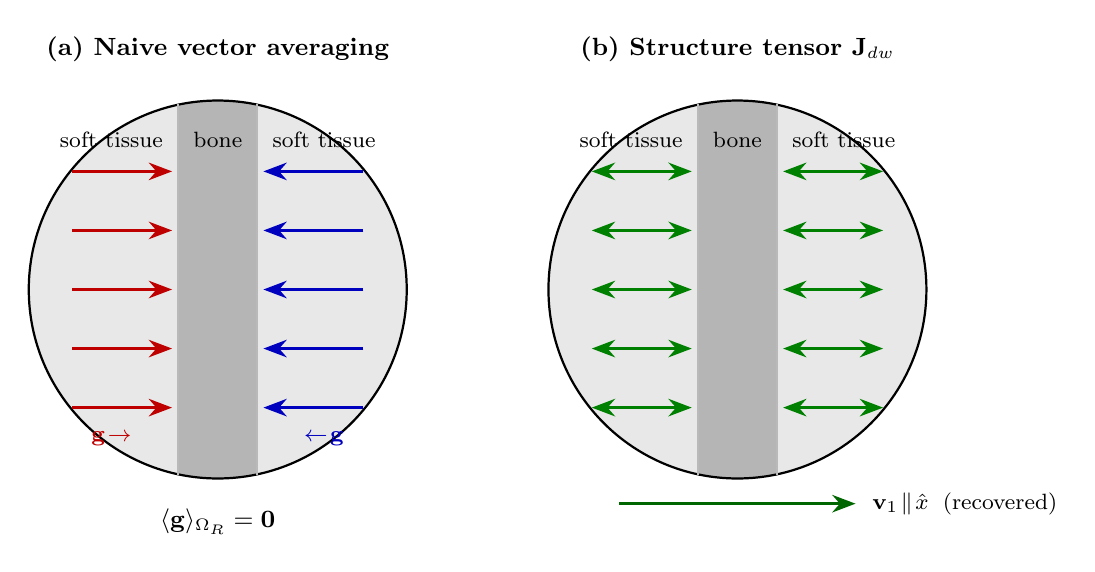
\begin{tikzpicture}[>=Stealth, thick, font=\small]

%% ===================== Panel (a): naive averaging =====================
\begin{scope}[xshift=0cm]

  % Filled regions, clipped to circle
  \begin{scope}
    \clip (0,0) circle (2.4cm);
    \fill[gray!18] (-3,-3) rectangle (3,3);       % soft tissue
    \fill[gray!58] (-0.5,-3) rectangle (0.5,3);   % bone slab
  \end{scope}
  \draw (0,0) circle (2.4cm);
  \draw[gray!55] (-0.5,-2.35) -- (-0.5, 2.35);
  \draw[gray!55] ( 0.5,-2.35) -- ( 0.5, 2.35);

  % LEFT face: tissue is on the left, bone on the right
  % => gradient in left tissue points RIGHTWARD (toward bone = higher HU)
  \foreach \y in {-1.5,-0.75,0,0.75,1.5}{
    \draw[->, red!75!black, line width=1.2pt] (-1.85,\y) -- (-0.58,\y);
  }

  % RIGHT face: bone is on the left, tissue is on the right
  % => gradient in right tissue points LEFTWARD (toward bone = higher HU)
  \foreach \y in {-1.5,-0.75,0,0.75,1.5}{
    \draw[->, blue!75!black, line width=1.2pt] (1.85,\y) -- (0.58,\y);
  }

  % Region labels (inside circle)
  \node[font=\footnotesize] at (-1.35, 1.90) {soft tissue};
  \node[font=\footnotesize] at ( 0,    1.90) {bone};
  \node[font=\footnotesize] at ( 1.35, 1.90) {soft tissue};

  % Arrow direction labels
  \node[red!75!black,  font=\footnotesize] at (-1.35,-1.90) {$\vg\!\rightarrow$};
  \node[blue!75!black, font=\footnotesize] at ( 1.35,-1.90) {$\leftarrow\!\vg$};

  % Result (below circle)
  \node at (0,-2.95) {$\langle\vg\rangle_{\Omega_R} = \mathbf{0}$};

  % Panel title
  \node[align=center, font=\small\bfseries] at (0, 3.05) {(a) Naive vector averaging};

\end{scope}

%% =================== Panel (b): structure tensor =====================
\begin{scope}[xshift=6.6cm]

  \begin{scope}
    \clip (0,0) circle (2.4cm);
    \fill[gray!18] (-3,-3) rectangle (3,3);
    \fill[gray!58] (-0.5,-3) rectangle (0.5,3);
  \end{scope}
  \draw (0,0) circle (2.4cm);
  \draw[gray!55] (-0.5,-2.35) -- (-0.5, 2.35);
  \draw[gray!55] ( 0.5,-2.35) -- ( 0.5, 2.35);

  % Outer-product contributions: UNSIGNED direction (double-headed arrows)
  % Both faces contribute identically -- the sign is squared away
  \foreach \y in {-1.5,-0.75,0,0.75,1.5}{
    \draw[<->, green!50!black, line width=1.2pt] (-1.85,\y) -- (-0.58,\y);
  }
  \foreach \y in {-1.5,-0.75,0,0.75,1.5}{
    \draw[<->, green!50!black, line width=1.2pt] (0.58,\y) -- (1.85,\y);
  }

  % Region labels
  \node[font=\footnotesize] at (-1.35, 1.90) {soft tissue};
  \node[font=\footnotesize] at ( 0,    1.90) {bone};
  \node[font=\footnotesize] at ( 1.35, 1.90) {soft tissue};

  % Dominant eigenvector shown below circle
  \draw[->, very thick, green!40!black] (-1.5,-2.72) -- (1.5,-2.72);
  \node[font=\footnotesize, right] at (1.5,-2.72)
    {$\;\mathbf{v}_1 \!\parallel\! \hat{x}$ \;(recovered)};

  % Panel title
  \node[align=center, font=\small\bfseries] at (0, 3.05) {(b) Structure tensor $\mathbf{J}_{dw}$};

\end{scope}

\end{tikzpicture}
\caption{Illustration of the gradient-vector cancellation problem and its
resolution via the structure tensor.
Both panels show a 2-D cross-section of the analysis sphere (circle); a thin
bone slab (dark grey) crosses the centre vertically, with soft tissue (light
grey) on both sides.
\textbf{(a)}~Red arrows: the Sobel gradient in the left soft-tissue region
points rightward into the bone (higher HU).
Blue arrows: the gradient in the right soft-tissue region points leftward,
also toward the bone.
Both sets are equal in magnitude but opposite in direction; their mean over
$\Omega_R$ is exactly zero, even though a strong, well-defined interface is
present.
\textbf{(b)}~Replacing each gradient vector $\vg$ with its outer product
$\vg\!\otimes\!\vg$ removes the sign: contributions from both faces become
identical (double-headed arrows).
Eigendecomposition of the accumulated $\mathbf{J}_{dw}$ correctly recovers
$\mathbf{v}_1 \parallel \hat{x}$ as the dominant edge normal.}
\label{fig:cancellation}
\end{figure}

\subsection{The Outer-Product Trick}

The solution is to represent each gradient not as a signed arrow but as a
\emph{direction preference} — a quantity that is the same for $\vg$ and
$-\vg$.

The mathematical object with this property is the \emph{outer product}
$\vg \otimes \vg$, a $3\times 3$ matrix:
\begin{equation}
    \vg \otimes \vg
    =
    \begin{pmatrix} G_z \\ G_y \\ G_x \end{pmatrix}
    \begin{pmatrix} G_z & G_y & G_x \end{pmatrix}
    =
    \begin{pmatrix}
        G_z^2   & G_z G_y & G_z G_x \\
        G_y G_z & G_y^2   & G_y G_x \\
        G_x G_z & G_x G_y & G_x^2
    \end{pmatrix}.
\end{equation}

The crucial observation is that squaring removes the sign:
$(-\vg)\otimes(-\vg) = \vg\otimes\vg$.
Left and right arrows — the two faces of the same boundary — now produce
\emph{identical} matrices and therefore reinforce rather than cancel when
summed.

\paragraph{Intuition.}
Think of it as a voting system.
Each voxel ``votes'' for the axis along which its gradient is most strongly
oriented.
The vote is not ``I point left'' or ``I point right'' (which would cancel),
but rather ``the variation here is along the $x$-direction'' — a statement
that is symmetric and thus consistent for both faces of the same interface.
Squaring the gradient components is exactly what turns a signed arrow into
this unsigned, direction-only vote.

\subsection{The Dose-Weighted Structure Tensor}

Summing the dose-weighted outer products over the analysis sphere gives the
\emph{dose-weighted structure tensor}:
\begin{equation}
    \boxed{
    \vJ_{dw}
    = \sum_{\vx \in \Omega_R} d(\vx)\,\vg(\vx)\otimes\vg(\vx)
    = \sum_{\vx \in \Omega_R} d(\vx)
        \begin{pmatrix}
            G_z^2   & G_z G_y & G_z G_x \\
            G_y G_z & G_y^2   & G_y G_x \\
            G_x G_z & G_x G_y & G_x^2
        \end{pmatrix}.
    }
    \label{eq:structure_tensor}
\end{equation}

$\vJ_{dw}$ is a $3\times3$ real symmetric matrix with non-negative diagonal
entries.
It is the dose-weighted accumulation of all gradient direction preferences
inside the sphere: every voxel contributes proportionally to both its local
dose and the squared strength of its edge.

\paragraph{What does $\vJ_{dw}$ encode?}
The diagonal entry $[\vJ_{dw}]_{zz} = \sum d(\vx)\,G_z^2$ records how
much dose-weighted gradient energy is oriented along the $z$-axis.
Similarly for $yy$ and $xx$.
The off-diagonal entry $[\vJ_{dw}]_{zy} = \sum d(\vx)\,G_z G_y$ records
correlations between the $z$- and $y$-components of the gradient: a large
positive value means gradients tend to be oriented in a direction that is
simultaneously in $z$ and in $y$, i.e.\ diagonally between the two axes.
The full $3\times3$ structure encodes the dominant orientation as a
\emph{shape in direction space}, not just a single number.

\subsection{Eigendecomposition: Reading the Shape of the Tensor}

A symmetric positive semi-definite matrix such as $\vJ_{dw}$ can be thought
of as defining an \emph{ellipsoid} in three-dimensional space.
The axes of the ellipsoid are the \emph{eigenvectors}; their lengths are the
square roots of the \emph{eigenvalues}.

\begin{equation}
    \vJ_{dw} = \vV\mLambda\vV^T,
    \qquad
    \mLambda = \mathrm{diag}(\lambda_1, \lambda_2, \lambda_3),
    \quad \lambda_1 \geq \lambda_2 \geq \lambda_3 \geq 0.
\end{equation}
The columns of $\vV = [\vv_1\;\vv_2\;\vv_3]$ are three mutually orthogonal
unit vectors — the principal directions of the gradient distribution.

\paragraph{Geometric picture.}
Imagine plotting one gradient arrow per voxel (each scaled by $\sqrt{d(\vx)}$)
as a point cloud in 3-D direction space.
The structure tensor captures the ``shape'' of this cloud:
\begin{itemize}
    \item If the cloud is elongated like a sausage — almost all arrows point
          along one direction — the ellipsoid is cigar-shaped: one long axis
          ($\lambda_1$ large) and two short axes ($\lambda_2$, $\lambda_3$
          small).
          This corresponds to a single dominant planar interface.
    \item If the cloud is spread equally in all directions — a sphere — all
          three eigenvalues are equal.
          This corresponds to edges pointing in every direction, e.g.\ a
          spherical bone inclusion.
    \item Intermediate cases (e.g.\ a cylindrical structure) produce a
          disc-like ellipsoid: one small axis ($\lambda_3$) and two large
          ones ($\lambda_1 \approx \lambda_2$).
\end{itemize}

\paragraph{Why does the long axis give the edge normal?}
At a sharp planar interface the gradient is large only in the direction
\emph{perpendicular} to the surface (because the CT intensity changes most
rapidly across the boundary).
All arrows therefore accumulate along this perpendicular direction: the cloud
is elongated exactly in the direction of the interface normal.
The long axis of the ellipsoid — eigenvector $\vv_1$ — is the dominant edge
normal.

\subsubsection*{Interpretation of eigenvectors and eigenvalues}

\begin{description}
    \item[$\vv_1$, $\lambda_1$:]
        The \emph{dominant edge normal} — the direction perpendicular to the
        most prominent tissue interface in the irradiated part of the sphere.
        A large $\lambda_1$ means the corresponding interface is strong and
        well-localised.

    \item[$\vv_3$, $\lambda_3$:]
        The direction \emph{along} the dominant edge (the tangential
        direction of least gradient variation).
        A small $\lambda_3$ relative to $\lambda_1$ confirms that the dominant
        interface is nearly planar.

    \item[$\vv_2$, $\lambda_2$:]
        The remaining principal direction, orthogonal to both.
        Together, $\vv_1$, $\vv_2$, $\vv_3$ form a complete orthonormal
        frame that describes the full 3-D geometry of the gradient
        distribution.
\end{description}

% ---------------------------------------------------------------------------
\section{Scalar Descriptors from the Structure Tensor}
\label{sec:scalar}
% ---------------------------------------------------------------------------

The structure tensor is a $3\times3$ matrix — too rich to use directly as a
regression feature or a comparison metric.
We extract three scalars that each capture a distinct, physically meaningful
aspect of the edge geometry.

\subsection{Edge Anisotropy}

\begin{equation}
    \boxed{A = \frac{\lambda_1 - \lambda_3}{\lambda_1 + \lambda_2 + \lambda_3}}
    \in [0,\,1]
    \label{eq:anisotropy}
\end{equation}

\paragraph{Intuition.}
Imagine comparing two objects: a rugby ball and a soccer ball.
The rugby ball has one long axis and two short ones — it is anisotropic.
The soccer ball looks the same from every direction — it is isotropic.
The anisotropy $A$ does exactly this comparison for the ellipsoid described
by the structure tensor.

\begin{description}
    \item[$A \approx 1$ (cigar-shaped ellipsoid):]
        $\lambda_1 \gg \lambda_2, \lambda_3$.
        Almost all dose-weighted gradient energy is concentrated along a
        single direction.
        This indicates one dominant, well-defined planar interface — for
        example, a flat bone plate crossing the sphere.
        The dominant edge normal $\vv_1$ is a reliable and meaningful
        descriptor in this case.

    \item[$A \approx 0$ (spherical ellipsoid):]
        $\lambda_1 \approx \lambda_2 \approx \lambda_3$.
        Gradient energy is spread uniformly across all directions.
        This indicates that the sphere contains many interfaces oriented in
        all directions (e.g.\ trabecular bone, or a spherical heterogeneity).
        There is no single dominant edge, and $\vv_1$ loses its meaning as a
        ``dominant normal'' — any direction would be equally valid.
\end{description}

A high anisotropy means both that the dominant edge is geometrically
well-defined \emph{and} that the angle $\theta$ (Section~\ref{sec:angle})
is a trustworthy number.
When $A$ is low, $\theta$ should be treated with caution.

\subsection{Dominant-Edge-to-Beam Angle}
\label{sec:angle}

The proton beam travels along the $z$-axis,
$\hat{z} = (1,0,0)^T$ in the $(z,y,x)$ convention used here.
The angle between the dominant edge normal $\vv_1$ and the beam is:
\begin{equation}
    \boxed{\theta = \arccos\!\bigl(|\vv_1 \cdot \hat{z}|\bigr)}
    \in [0^\circ,\,90^\circ]
    \label{eq:beam_angle}
\end{equation}

The absolute value is necessary because the sign of an eigenvector is
arbitrary: $\vv_1$ and $-\vv_1$ describe the same geometric direction, but
would give dot products of opposite sign without the absolute value.

\paragraph{Intuition: the wall and the ball.}
Imagine throwing a ball along a corridor and asking how much a wall inside
the corridor slows it down.
\begin{itemize}
    \item If the wall is placed \emph{across} the corridor (perpendicular to
          the ball's path), the ball hits the wall straight on — maximum
          interaction.
    \item If the wall runs \emph{along} the corridor (parallel to the ball's
          path), the ball flies past it with minimal disturbance.
\end{itemize}
The angle $\theta$ is exactly this: it measures how much the dominant tissue
interface is ``across the corridor'' of the proton beam.

\paragraph{Physical interpretation.}
In proton therapy, the energy deposited by a pencil beam at depth depends
on the \emph{water-equivalent path length} (WEPL) through the materials
along the beam axis.
A tissue interface changes the WEPL only insofar as it \emph{crosses} the
beam path.

\begin{description}
    \item[$\theta \approx 0^\circ$ (interface perpendicular to beam):]
        The edge normal is parallel to $\hat{z}$.
        The beam must pass through the interface.
        Each proton traverses a step change in density, shifting the
        Bragg-peak depth.
        This is the configuration of maximum range uncertainty and is
        most likely to degrade model prediction accuracy.

    \item[$\theta \approx 90^\circ$ (interface parallel to beam):]
        The edge normal is perpendicular to $\hat{z}$.
        The interface runs alongside the beam without being crossed.
        The WEPL and therefore the Bragg-peak depth are less perturbed;
        any residual effect is on the lateral dose profile rather than
        the range.
\end{description}

\subsection{Total Edge Energy}

\begin{equation}
    \boxed{E_{total} = \mathrm{tr}(\vJ_{dw}) = \lambda_1 + \lambda_2 + \lambda_3
           = \sum_{\vx \in \Omega_R} d(\vx)\,\norm{\vg(\vx)}^2}
    \label{eq:total_energy}
\end{equation}

The trace of the structure tensor equals the dose-weighted sum of squared
gradient magnitudes.
This identity follows directly from the definition~\eqref{eq:structure_tensor}:
the diagonal entries of $\vg\otimes\vg$ are $G_z^2$, $G_y^2$, $G_x^2$,
whose sum is $\norm{\vg}^2$.

$E_{total}$ is the dose-weighted analogue of the existing
\texttt{sum\_sobel\_bp} metric (which uses unsquared magnitudes and no dose
weighting).
Its advantage is that it decomposes cleanly into the three eigenvalues,
making it consistent with the rest of the structure-tensor framework.

\paragraph{Relationship between $E_{total}$ and $A$.}
The two metrics are complementary.
$E_{total}$ tells you \emph{how much} total edge energy is present in the
irradiated region; $A$ tells you \emph{how concentrated} that energy is
along one direction.
A sphere with a single sharp bone plate and a sphere filled with fine
trabecular bone could have similar $E_{total}$, but very different $A$:
the bone plate gives $A \approx 1$, the trabecular bone gives $A \approx 0$.

% ---------------------------------------------------------------------------
\section{Summary of Proposed Metrics}
% ---------------------------------------------------------------------------

\begin{table}[h!]
    \centering
    \caption{Proposed dose-weighted Sobel metrics.
             All quantities are computed inside the analysis sphere
             $\Omega_R$ centred on the Bragg peak.}
    \label{tab:metrics}
    \begin{tabular}{llp{7cm}}
        \toprule
        Symbol & Equation & Physical meaning \\
        \midrule
        $\bar{S}_{dw}$  & \eqref{eq:dw_mean}
            & Dose-weighted mean Sobel gradient magnitude.
              Overall edge intensity in the irradiated region. \\
        $\vJ_{dw}$      & \eqref{eq:structure_tensor}
            & Dose-weighted structure tensor ($3\times3$ matrix). \\
        $\vv_1$         & eigenvector of $\vJ_{dw}$, $\lambda_1$
            & Dominant edge normal direction (3-D unit vector). \\
        $A$             & \eqref{eq:anisotropy}
            & Edge anisotropy: how planar vs.\ omnidirectional the
              dominant interface is. \\
        $\theta$        & \eqref{eq:beam_angle}
            & Angle between dominant edge normal and beam axis;
              directly related to range-uncertainty risk. \\
        $E_{total}$     & \eqref{eq:total_energy}
            & Dose-weighted total edge energy (trace of $\vJ_{dw}$). \\
        \bottomrule
    \end{tabular}
\end{table}

% ---------------------------------------------------------------------------
\section{Implementation Notes}
% ---------------------------------------------------------------------------

\begin{enumerate}
    \item \textbf{Dose volume.}
          At training/analysis time, the ground-truth dose $d(\vx)$ is used
          for weighting.
          When the metrics are applied post-hoc to model predictions, the
          predicted dose could be substituted; the choice should be documented
          per experiment.

    \item \textbf{Sphere extraction.}
          The current implementation computes Sobel on the full CT volume and
          then masks.
          This remains correct for the structure tensor; only the accumulation
          step changes.

    \item \textbf{Numerical stability.}
          If $\sum_{\vx \in \Omega_R} d(\vx) < \varepsilon_{tol}$ (no dose
          in sphere), all metrics default to zero and $\vv_1$ is undefined.
          The anisotropy $A$ should also be set to zero in this case.

    \item \textbf{Eigendecomposition.}
          $\vJ_{dw}$ is a $3\times3$ real symmetric matrix.
          \texttt{numpy.linalg.eigh} provides an efficient, numerically stable
          decomposition with eigenvalues guaranteed to be real and returned in
          ascending order (reverse to get descending $\lambda_1 \geq \lambda_2
          \geq \lambda_3$).

    \item \textbf{Sign convention for $\vv_1$.}
          The eigenvector sign is arbitrary.
          The beam-edge angle~\eqref{eq:beam_angle} uses the absolute value of
          the dot product, making it sign-invariant.
          If the vector itself is stored or visualised, a canonical sign
          convention should be chosen (e.g.\ $v_{1,z} \geq 0$).
\end{enumerate}

% ---------------------------------------------------------------------------
\section{Comparison of Method DW and Method TH}
\label{sec:comparison}
% ---------------------------------------------------------------------------

\subsection{What Each Method Assumes}

Before designing experiments it is worth stating explicitly what each method
assumes about the relationship between dose and edge relevance.

\textbf{Method DW} assumes that \emph{the relevance of a tissue interface scales
continuously with the local dose}.
A voxel receiving twice the dose of a neighbour contributes twice as much to
the metric.
This is a soft, graded view: there is no sharp boundary between
``relevant'' and ``irrelevant''; every dose-positive voxel matters to some
degree.

\textbf{Method TH} assumes that \emph{there is a hard clinical boundary between
irradiated and unirradiated tissue}, defined by the 5\,\% global isodose
surface.
Once a voxel is classified as irradiated, it is treated as equally relevant
regardless of its actual dose value.
This is a binary view that aligns with standard radiotherapy dose prescription
concepts.

The two assumptions lead to different behaviours in specific geometric
configurations, summarised in Table~\ref{tab:method_differences}.

\begin{table}[h!]
    \centering
    \caption{Expected behaviour of Method DW and Method TH in representative
             geometric configurations.}
    \label{tab:method_differences}
    \begin{tabular}{>{\raggedright\arraybackslash}p{4.5cm}
                    >{\raggedright\arraybackslash}p{4.5cm}
                    >{\raggedright\arraybackslash}p{4.5cm}}
        \toprule
        Scenario & Method DW & Method TH \\
        \midrule
        Interface well inside the high-dose region
        & Up-weighted; contributes strongly
        & Included; contributes equally \\[4pt]
        Interface near the 5\,\% isodose surface
        & Down-weighted by low dose; contributes little
        & Either fully included or fully excluded \\[4pt]
        All dose in the sphere is uniform (flat dose plateau)
        & Equivalent to unweighted mean over sphere
        & Equivalent to unweighted mean over thresholded sphere \\[4pt]
        Highly peaked dose (narrow Bragg peak)
        & Strongly up-weights voxels near the dose maximum
        & Treats all above-threshold voxels equally \\
        \bottomrule
    \end{tabular}
\end{table}

\subsection{Metrics to Be Compared}

For every sample in the training set, both methods are computed for all
scalar descriptors.
Table~\ref{tab:comparison_metrics} lists the full set of paired quantities.

\begin{table}[h!]
    \centering
    \caption{Scalar descriptors computed under each method.
             All quantities are extracted from the analysis sphere $\Omega_R$.}
    \label{tab:comparison_metrics}
    \begin{tabular}{lll}
        \toprule
        Descriptor & Method DW & Method TH \\
        \midrule
        Mean gradient magnitude & $\bar{S}_{DW}$~\eqref{eq:dw_mean}
                                & $\bar{S}_{TH}$~\eqref{eq:th_mean} \\
        Edge anisotropy         & $A_{DW}$
                                & $A_{TH}$ \\
        Beam-edge angle         & $\theta_{DW}$
                                & $\theta_{TH}$ \\
        Total edge energy       & $E_{DW}$
                                & $E_{TH}$ \\
        \bottomrule
    \end{tabular}
\end{table}

\subsection{Comparison Protocol}

The comparison is structured around three complementary analyses.

\subsubsection{Correlation with Model Error}

For each descriptor and each method, compute the Spearman rank correlation
$\rho$ with the model prediction error, measured by:
\begin{itemize}
    \item Gamma pass rate (GPR) at 3\,\%/3\,mm — primary endpoint;
    \item RMSE and MAPE — secondary endpoints.
\end{itemize}

Because we have eight descriptor-method combinations ($4 \times 2$), we
report all correlations in a single table, comparing $\rho_{DW}$ and
$\rho_{TH}$ side by side for each descriptor.
A statistically significant difference in $|\rho|$ between the two methods
for the same descriptor indicates that the weighting strategy matters for
that descriptor.

\subsubsection{Ranking Consistency}

Even if both methods have similar correlation with model error, they may
disagree on which individual samples are the most heterogeneous.
To quantify this, compute Kendall's rank correlation coefficient $\tau$
between the DW and TH rankings for each descriptor:
\begin{equation}
    \tau = \frac{\#\,\text{concordant pairs} - \#\,\text{discordant pairs}}
               {\tfrac{1}{2}N(N-1)},
\end{equation}
where $N$ is the number of samples.

$\tau \approx 1$ means the two methods produce nearly identical rankings;
$\tau \approx 0$ means they are essentially independent.
Low $\tau$ for a given descriptor signals that the weighting choice is
consequential and that one method must be selecting genuinely different
information than the other.

\subsubsection{Discordance Analysis}
\label{sec:discordance}

Identify the $k = 10$ samples with the largest absolute rank difference
$|\mathrm{rank}_{DW} - \mathrm{rank}_{TH}|$ for the primary descriptor
$\bar{S}$.
For each discordant sample, examine:
\begin{enumerate}
    \item The dose distribution inside $\Omega_R$: is it narrowly peaked (Bragg
          peak well inside the sphere) or broadly spread?
    \item The active set size $|\Omega_R^{TH}|$ relative to $|\Omega_R|$: what
          fraction of the sphere falls above the global 5\,\% threshold?
    \item Whether the tissue interface responsible for the high Sobel magnitude
          overlaps with the high-dose zone or lies in the periphery of the
          sphere.
\end{enumerate}

This analysis reveals the geometric conditions under which the two methods
diverge and provides a physical interpretation of the discordance.

\subsection{Expected Sources of Discordance}

Two structural differences between the methods generate predictable
discordances:

\paragraph{Dose-peak localisation.}
When the Bragg peak is sharp and sits near the centre of the sphere, the
dose is highly concentrated over a small number of voxels.
Method DW up-weights those voxels strongly.
If the dominant interface happens to be at the dose peak, Method DW gives it
disproportionately high weight relative to Method TH.
Conversely, if the dominant interface is at the sphere boundary where dose is
low, Method DW suppresses it while Method TH may still include it (provided
the dose there exceeds 5\,\% of the global maximum).

\paragraph{Global vs.\ local threshold reference.}
Method TH's threshold is anchored to the global dose maximum $d_{\mathrm{grid}}$,
which is consistent across samples but may include or exclude very different
fractions of the sphere depending on the absolute dose level.
A low-energy beam (small $d_{\mathrm{grid}}$) may have most of the sphere above
threshold; a high-energy beam with a narrow Bragg peak may have very few
voxels above it.
Method DW is immune to this variation because it normalises by the local dose
sum $\sum_{\vx \in \Omega_R} d(\vx)$.

\subsection{Decision Criterion}

The preferred method will be selected based on the following ordered criteria:
\begin{enumerate}
    \item \textbf{Predictive power}: the method with higher $|\rho|$ with GPR
          for the majority of descriptors is preferred.
    \item \textbf{Consistency}: in the case of comparable predictive power,
          prefer the method with more stable behaviour across the discordant
          samples identified in Section~\ref{sec:discordance}.
    \item \textbf{Interpretability}: Method TH has a direct clinical
          interpretation (5\,\% isodose surface); Method DW has a cleaner
          mathematical formulation.
          This criterion is used as a tiebreaker.
\end{enumerate}

\end{document}
